
\begin{figure}
  \centering

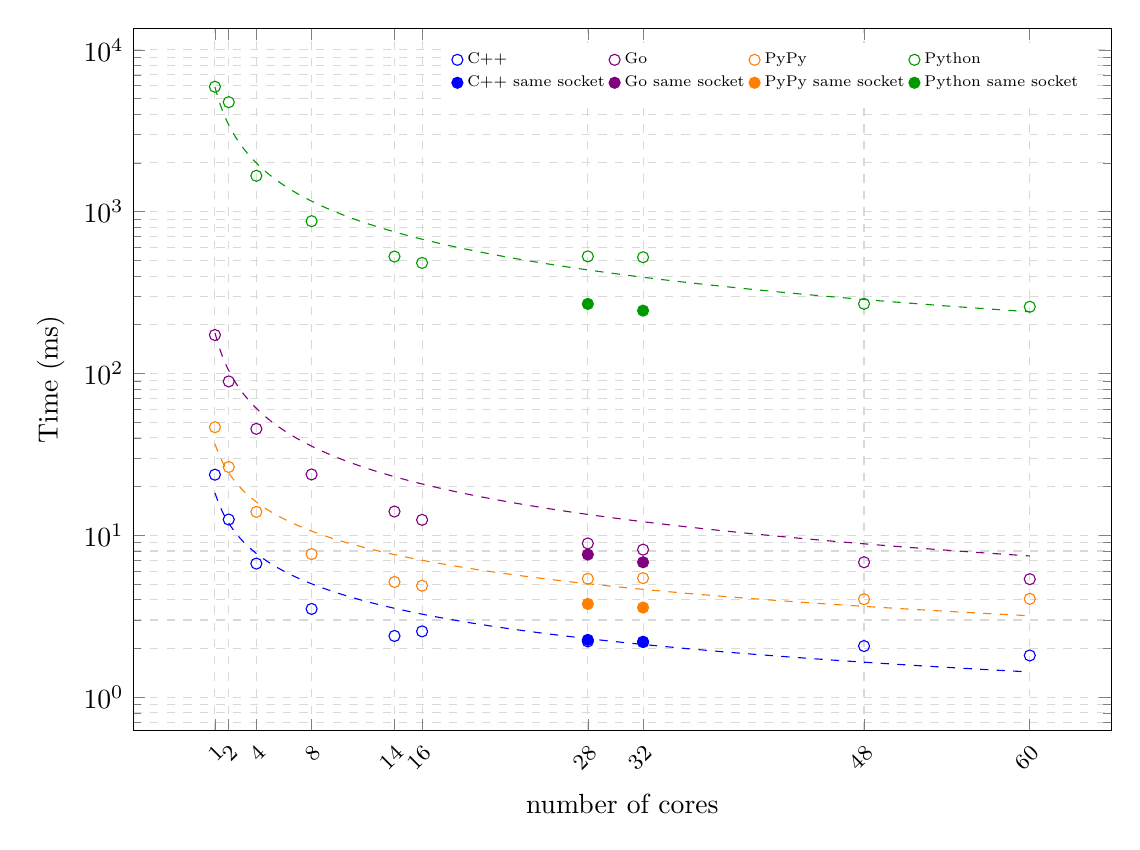
\begin{tikzpicture}
  \begin{semilogyaxis}[
      width=14cm,
      height=10.5cm,
      xlabel={number of cores},
      ylabel={Time (ms)},
      ymode=log,
      xmode=linear,
      grid=both,
      minor tick num=1,
      grid style={gray!30,dashed},
      xtick={1,2,4,8,14,16,28,32,48,60},
      x tick label style={
        font=\footnotesize,
        rotate=45,
        anchor=north east
      },
      legend style={
        at={(0.98,0.98)},
        anchor=north east,
        font=\scriptsize,
        nodes={scale=0.8,transform shape},
        draw=none
      },
      legend columns=2,
      transpose legend,
      legend cell align=left,
    ]

    %% C++ %%
    \addplot[
      blue,
      only marks,
      mark=o,
      mark options={draw=blue,fill=white}
    ]
    table[row sep=\\] {
      x    y \\
      1    23.70  \\
      2    12.52  \\
      4    6.69   \\
      8    3.51   \\
      14   2.39   \\
      16   2.55   \\
      28   2.21   \\
      32   2.20   \\
      48   2.07   \\
      60   1.81   \\
    };
    \addlegendentry{C++}

    \addplot[
      blue,
      only marks,
      mark=*,
      mark options={draw=blue,fill=blue}
    ]
    table[row sep=\\] {
      x    y \\
      28   2.26   \\
      32   2.19   \\
    };
    \addlegendentry{C++ same socket}

    % power‐law fit: y = 18.3 * x^(-0.6223)
    \addplot[
      blue,
      dashed,
      forget plot,
      domain=1:60,
      samples=200
    ] {18.3 * x^(-0.6223)};

    %% Go %%
    \addplot[
      violet,
      only marks,
      mark=o,
      mark options={draw=violet,fill=white}
    ]
    table[row sep=\\] {
      x    y \\
      1    172.95 \\
      2    89.32  \\
      4    45.51  \\
      8    23.78  \\
      14   14.03  \\
      16   12.46  \\
      28   8.91   \\
      32   8.16   \\
      48   6.82   \\
      60   5.36   \\
    };
    \addlegendentry{Go}

    \addplot[
      violet,
      only marks,
      mark=*,
      mark options={draw=violet,fill=violet}
    ]
    table[row sep=\\] {
      x    y \\
      28   7.61  \\
      32   6.82  \\
    };
    \addlegendentry{Go same socket}

    % power‐law fit: y = 178.3 * x^(-0.7753)
    \addplot[
      violet,
      dashed,
      forget plot,
      domain=1:60,
      samples=200
    ] {178.3 * x^(-0.7753)};

    %% PyPy %%
    \addplot[
      orange,
      only marks,
      mark=o,
      mark options={draw=orange,fill=white}
    ]
    table[row sep=\\] {
      x    y \\
      1    46.58  \\
      2    26.43  \\
      4    13.97  \\
      8    7.66   \\
      14   5.15   \\
      16   4.88   \\
      28   5.39   \\
      32   5.44   \\
      48   4.03   \\
      60   4.05   \\
    };
    \addlegendentry{PyPy}

    \addplot[
      orange,
      only marks,
      mark=*,
      mark options={draw=orange,fill=orange}
    ]
    table[row sep=\\] {
      x    y \\
      28   3.77   \\
      32   3.58   \\
    };
    \addlegendentry{PyPy same socket}

    % power‐law fit: y = 36.8 * x^(-0.5976)
    \addplot[
      orange,
      dashed,
      forget plot,
      domain=1:60,
      samples=200
    ] {36.8 * x^(-0.5976)};

    %% Python %%
    \addplot[
      green!60!black,
      only marks,
      mark=o,
      mark options={draw=green!60!black,fill=white}
    ]
    table[row sep=\\] {
      x    y \\
      1    5913.41  \\
      2    4749.55  \\
      4    1665.41  \\
      8    872.89   \\
      14   528.12   \\
      16   482.30   \\
      28   529.22   \\
      32   523.04   \\
      48   269.41   \\
      60   258.44   \\
    };
    \addlegendentry{Python}

    \addplot[
      green!60!black,
      only marks,
      mark=*,
      mark options={draw=green!60!black,fill=green!60!black}
    ]
    table[row sep=\\] {
      x    y \\
      28   269.13  \\
      32   244.57  \\
    };
    \addlegendentry{Python same socket}

    % power‐law fit: y = 5894 * x^(-0.7811)
    \addplot[
      green!60!black,
      dashed,
      forget plot,
      domain=1:60,
      samples=200
    ] {5894 * x^(-0.7811)};

  \end{semilogyaxis}
\end{tikzpicture}

\caption{Execution time of the server in Joules for different core configurations}
  \label{fig:server-execution-time}
\end{figure}

\begin{table}[ht]
    \centering
    \begin{tabular}{lrrrr}
        \hline
        time         & C++             & Go            & PyPy          & Python     \\
        \hline
        1            & 23.70           & 172.95        & 46.58         & 5,913.41        \\
        2            & 12.52           & 89.32         & 26.43         & 4,749.55        \\
        4            & 6.69            & 45.51         & 13.97         & 1,665.41        \\
        8	           & 3.51  	         & 23.78 	       & 7.66          & 872.89          \\
        14           & 2.39            & 14.03         & 5.15          & 528.12          \\
        16           & 2.55            & 12.46         & 4.88          & 482.30          \\
        28           & 2.21            & 8.91          & 5.39          & 529.22          \\
        28 same CPU  & 2.26            & 7.61          & 3.77          & 269.13          \\
        32           & 2.20            & 8.16          & 5.44          & 523.04          \\
        32 same CPU  & 2.19            & 6.82          & 3.58          & \textbf{244.57} \\
        48           & 2.07            & 6.82          & 4.03          & 269.41          \\
        60           & \textbf{1.81}   & \textbf{5.36} & \textbf{4.05} & 258.44          \\
        \hline
    \end{tabular}
    \caption{Execution time by implementation and core count}
    \label{tab:server-execution-time}
\end{table}
